\documentclass[a4paper,12pt]{article}

\usepackage{cmap}
\usepackage{mathtext}
\usepackage[T2A]{fontenc}
\usepackage[utf8]{inputenc}
\usepackage[english,russian]{babel}

\usepackage{indentfirst}


\usepackage{amsmath,amsfonts,amssymb,amsthm,mathtools}
\usepackage{icomma}

\usepackage{euscript}
\usepackage{mathrsfs}

\usepackage[left=25mm, top=20mm, right=25mm, bottom=20mm, nohead]{geometry}

\usepackage{dirtree}

\DeclareMathOperator{\sgn}{\mathop{sgn}}





\begin{document}

\begin{titlepage}

\thispagestyle{empty}
\centerline{\Large{Нацональный иследовательскиий университет ИТМО}}
\centerline{\Large{Факультет инфокоммункацонных систем}}
\centerline{\Large{и технологий}}

\vfill

\centerline{\huge{Лабораторная работа №1}}
\vspace{0.5cm}
\centerline{\Large{Введение в web-разработку}}

\vfill

Студент группы К33212 \hfill Шелягов А.С.

Преподаватель \hfill Марченко Е.В.

\vfill

\centerline{Санкт-Петербург, 2023}
\clearpage
\end{titlepage}


\section{Цель работы.}

Познакомится с основами создания web-страниц, использующих
HTML, стили и код JavaScript и не требующими обмена данными с сервером.


\section{Выполнение заданий}

\subsection{Упражнение 1.  Создание простой html-страницы}
По примеру из методички был создан html-файл, результат запуска которого представлен ниже(рис.1):
\begin{figure}[!h]
\begin{center}
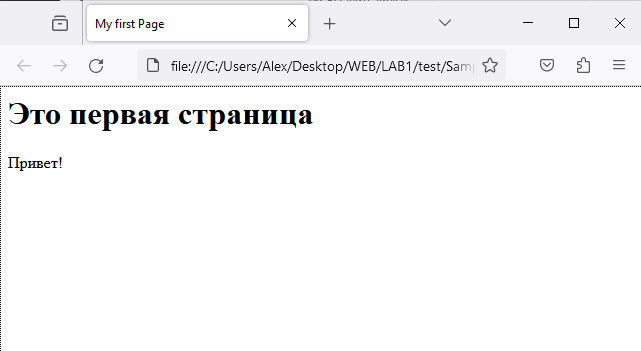
\includegraphics[scale=0.7]{pic1.png}
\caption{Результат запуска \textbf{Sample01.html}}
\end{center}
\end{figure}

\subsection{Упражнение 2.  Использование стилей для оформления страниц}
По примеру из методички в html-файл был добавлен парный тег \textbf{<style>}, в котором прописаны изменения цветов фона страницы  текста внутри парного тега \textbf{<p>} . Результат запуска представлен ниже(рис.2):
\begin{figure}[!h]
\begin{center}
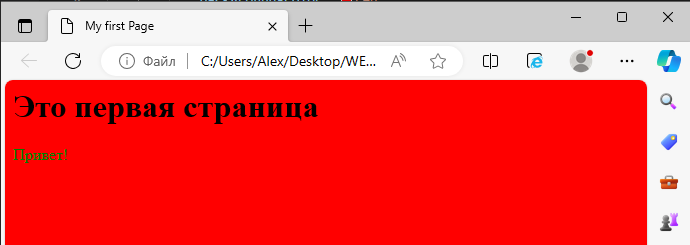
\includegraphics[scale=0.7]{pic2.png}
\caption{Результат запуска \textbf{Sample02.html}}
\end{center}
\end{figure}

\subsection{Упражнение 3.  Подключение кода javascript на html-страницу}
По примеру из методички в html-файл был добавлен парный тег \textbf{<script>}, в котором прописан вызов оповещенияg при загрузке страницы. Результат запуска  представлен ниже(рис.3):
\begin{figure}[!h]
\begin{center}
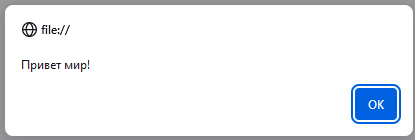
\includegraphics[scale=1]{pic3.png}
\caption{Результат запуска \textbf{Sample03.html}}
\end{center}
\end{figure}


\section{Выводы.}

В результате выполнениия лабораторной работы были созданы 3 html-файла, которые демонстрируют работу важнейщих html-тегов, а также работу тегов  \textbf{<style>} и \textbf{<script>}. Ниже представлено дерево рабочей директории: \\
\dirtree{%
.1 /.
.2 Sample01.html.
.2 Sample02.html.
.2 Sample03.html.
}


\end{document}